% Ebene Welle: E (x), B (y), S = E x B / mu0 in Ausbreitungsrichtung z
% Gemeinsamer Stil für alle Abbildungen (TikZ -> SVG, siehe figures/build.mjs).
%
% Farben sind Platzhalter ("Sentinels"): build.mjs ersetzt sie im SVG durch
% CSS-Variablen, damit die Abbildungen im hellen und dunklen Modus passen.
% Andere Farben (auch schwarz/weiß) bricht der Build mit Fehler ab.
%
%   fg    Linien, Beschriftung          -> --dark
%   mu    Hilfslinien, Achsen, Maße      -> --gray
%   acc   das eine Konzept der Abbildung -> --secondary (Lime/Oliv)
%   blue  zweite Größe, negative Ladung  -> --fig-blue
%   warm  dritte Größe, positive Ladung  -> --fig-warm
%   bg    Seitenhintergrund (Aussparen)  -> --light
%
% Kein \clip verwenden: pdftocairo macht daraus Clip-Gruppen, in denen exakt
% waagerechte/senkrechte Linien verschwinden. Berechnete Kurven schneidet
% gen/*.py selbst am Rahmen ab.
\documentclass[tikz,border=3pt]{standalone}
\usepackage{amsmath,amssymb,bm}
% Text serifenlos wie die Seite, Mathe in Computer Modern wie KaTeX
\renewcommand{\familydefault}{\sfdefault}
\usetikzlibrary{arrows.meta,calc,decorations.markings,patterns,3d,positioning,angles,quotes}

\definecolor{fg}{RGB}{1,2,3}
\definecolor{mu}{RGB}{4,5,6}
\definecolor{acc}{RGB}{7,8,9}
\definecolor{blue}{RGB}{10,11,12}
\definecolor{warm}{RGB}{13,14,15}
\definecolor{bg}{RGB}{16,17,18}

% Vektoren wie auf der Website (KaTeX \mathbf)
\newcommand{\vv}[1]{\mathbf{#1}}

\tikzset{
  every picture/.style={fg, line width=0.8pt, line cap=round, line join=round,
    >={Stealth[length=5.5pt,width=4.4pt]}},
  every node/.style={font=\small},
  % Linientypen
  main/.style={line width=0.9pt},
  thin/.style={line width=0.5pt},
  aux/.style={mu, line width=0.5pt, dash pattern=on 2.5pt off 2pt},
  axis/.style={mu, line width=0.6pt, ->},
  vec/.style={line width=1.1pt, ->},
  field/.style={line width=0.7pt, postaction={decorate},
    decoration={markings, mark=at position #1 with {\arrow{Stealth[length=4.5pt,width=3.6pt]}}}},
  field/.default=0.5,
  % Flächen
  soft/.style={fill=#1, fill opacity=0.14},
  soft/.default=acc,
  % Ladungen
  qpos/.style={circle, fill=warm, inner sep=0pt, minimum size=9pt,
    path picture={\draw[bg, line width=0.9pt] ($(path picture bounding box.center)+(-2pt,0)$) -- +(4pt,0)
      ($(path picture bounding box.center)+(0,-2pt)$) -- +(0,4pt);}},
  qneg/.style={circle, fill=blue, inner sep=0pt, minimum size=9pt,
    path picture={\draw[bg, line width=0.9pt] ($(path picture bounding box.center)+(-2pt,0)$) -- +(4pt,0);}},
  dot/.style={circle, fill=fg, inner sep=0pt, minimum size=3pt},
  % Beschriftung mit Aussparung, damit Linien den Text nicht kreuzen
  lbl/.style={fill=bg, inner sep=1.5pt},
  % Icons: kräftigere Linien, keine Schrift
  icon/.style={line width=1.6pt, >={Stealth[length=6pt,width=5pt]}},
}

\begin{document}
% Projektion: z nach rechts, x nach oben, y aus der Ebene (schräg nach vorn-unten).
% Rechtshändig: x (oben) × y (vorn) = z (rechts).
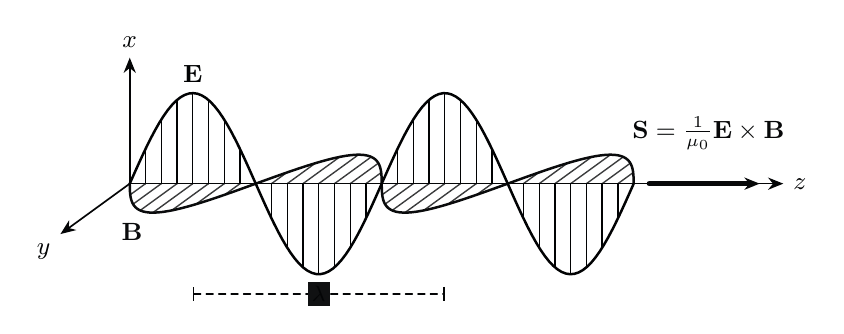
\begin{tikzpicture}[x={(0,1cm)}, y={(-0.55cm,-0.4cm)}, z={(1cm,0)}]
  \def\L{6.4} \def\lam{3.2} \def\A{1.15}
  \draw[axis] (0,0,0) -- (0,0,\L+1.9) node[anchor=west, text=fg] {$z$};
  \draw[axis] (0,0,0) -- (1.6,0,0) node[anchor=south, text=fg] {$x$};
  \draw[axis] (0,0,0) -- (0,1.6,0) node[anchor=north east, text=fg] {$y$};
  % B in der yz-Ebene (hinten zuerst zeichnen)
  \foreach \k in {1,...,32} {
    \pgfmathsetmacro{\zz}{\k*\L/32}
    \draw[blue, thin, opacity=0.8] (0,0,\zz) -- (0,{\A*0.8*sin(360*\zz/\lam)},\zz);
  }
  \draw[blue, main, domain=0:\L, samples=120, variable=\t] plot (0,{\A*0.8*sin(360*\t/\lam)},\t);
  % E in der xz-Ebene
  \foreach \k in {1,...,32} {
    \pgfmathsetmacro{\zz}{\k*\L/32}
    \draw[fg, thin] (0,0,\zz) -- ({\A*sin(360*\zz/\lam)},0,\zz);
  }
  \draw[fg, main, domain=0:\L, samples=120, variable=\t] plot ({\A*sin(360*\t/\lam)},0,\t);
  % Beschriftung am ersten Maximum z = lambda/4
  \node[anchor=south] at (\A,0,\lam/4) {$\vv E$};
  \node[blue, anchor=north east] at (0,\A*0.8,\lam/4) {$\vv B$};
  % Poynting-Vektor
  \draw[vec, acc, line width=2pt] (0,0,\L+0.2) -- (0,0,\L+1.6);
  \node[acc, anchor=south] at (0.3,0,\L+0.95) {$\vv S=\tfrac{1}{\mu_0}\vv E\times\vv B$};
  % Wellenlänge
  \draw[aux, |-|] (-\A-0.25,0,\lam/4) -- node[lbl, text=mu, font=\footnotesize] {$\lambda$} (-\A-0.25,0,\lam/4+\lam);
\end{tikzpicture}
\end{document}
